\documentclass[tikz,border=3pt]{standalone}
\usepackage{amsmath}
\usetikzlibrary{arrows.meta,patterns,positioning}
\definecolor{ohred}{HTML}{B23B2E}
\definecolor{rcblue}{HTML}{2F5FA6}
\definecolor{warm}{HTML}{E68A2E}
\tikzset{
  meshup/.style={fill=black!16, fill opacity=0.20, draw=black!34, draw opacity=0.44, line width=0.22pt},
  meshdown/.style={fill=black!26, fill opacity=0.20, draw=black!36, draw opacity=0.44, line width=0.22pt},
  meshside/.style={fill=black!9, fill opacity=0.17, draw=black!30, draw opacity=0.42, line width=0.22pt},
  selectedface/.style={fill=ohred!52, fill opacity=0.78, draw=ohred!88!black, draw opacity=0.96, line width=0.75pt},
  plate/.style={fill=black!4, fill opacity=0.22, draw=black!35, draw opacity=0.55, line width=0.5pt, pattern=north east lines, pattern color=black!25},
  sampleray/.style={->, >=Latex, dash pattern=on 2.2pt off 2.2pt, line width=0.95pt, ohred!82!black},
  axis/.style={->, >=Latex, line width=1.15pt, black!70},
  srcdot/.style={ohred!85!black},
  paneltitle/.style={font=\bfseries\large, text=black!82},
  meshlabel/.style={font=\bfseries, text=black!82},
  formulabox/.style={draw=black!35, fill=black!3, rounded corners=2pt, inner xsep=7pt, inner ysep=5pt, font=\large},
  resultbox/.style={draw=ohred!70!black, fill=ohred!8, rounded corners=2pt, inner xsep=7pt, inner ysep=5pt, font=\bfseries},
  textblock/.style={font=\normalsize, text=black!82},
  smalltext/.style={font=\small, text=black!72},
  notebox/.style={font=\small, text=black!72, align=left, draw=black!18, fill=black!2, rounded corners=2pt, inner xsep=5pt, inner ysep=4pt},
  barbase/.style={line width=5.5pt, black!15},
  barsegA/.style={line width=5.5pt, rcblue!75},
  barsegB/.style={line width=5.5pt, warm!85},
  barsegC/.style={line width=5.5pt, ohred!76},
  tick/.style={line width=0.55pt, black!55},
}
\begin{document}
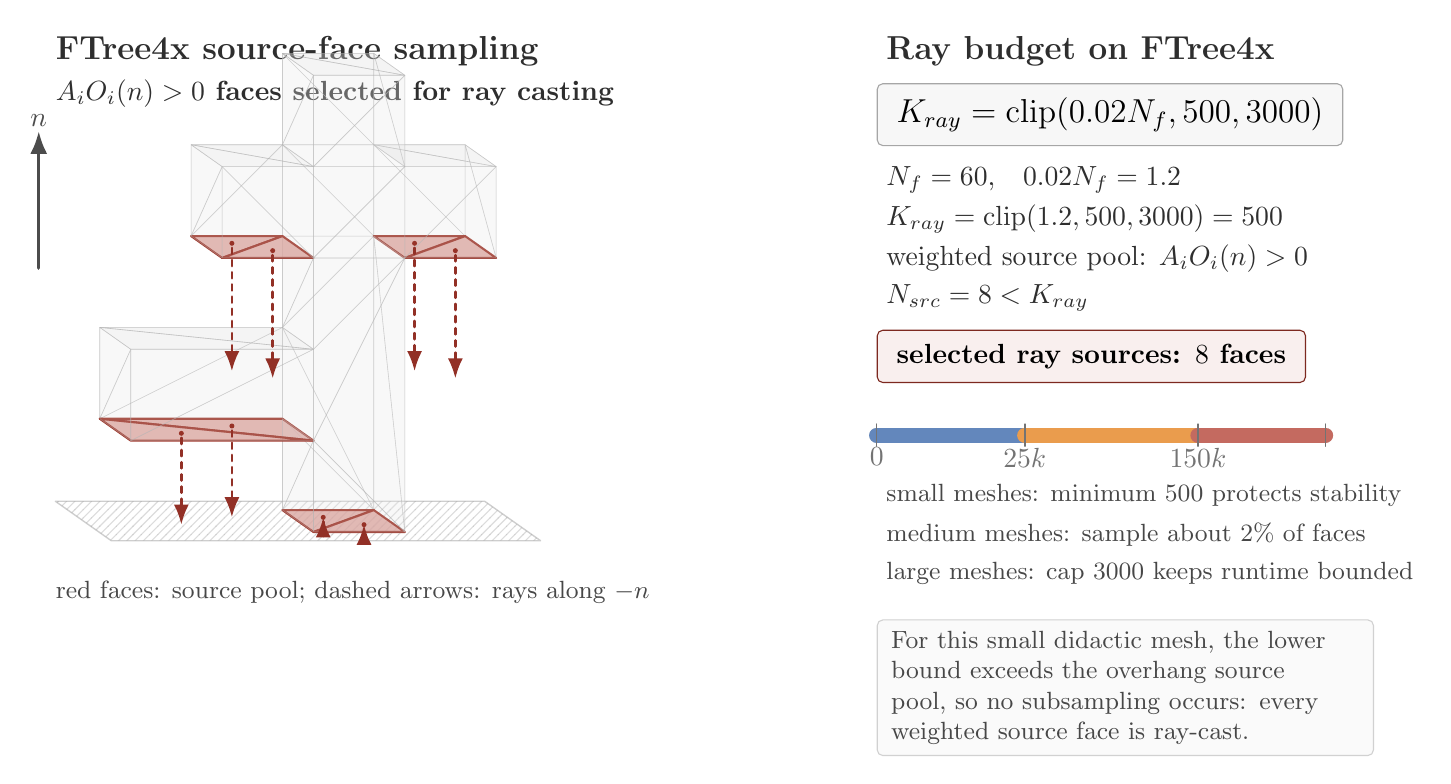
\begin{tikzpicture}[line join=round,line cap=round]
\node[paneltitle,anchor=west] at (-3.2,6.35) {FTree4x source-face sampling};
\node[meshlabel,anchor=west] at (-3.2,5.82) {$A_iO_i(n)>0$ faces selected for ray casting};
\filldraw[plate] (-3.081,0.640) -- (2.371,0.640) -- (3.081,0.139) -- (-2.371,0.139) -- cycle;
\filldraw[meshside] (-2.517,1.688) -- (-0.197,1.688) -- (-0.197,2.848) -- cycle;
\filldraw[meshside] (-2.517,1.688) -- (-0.197,2.848) -- (-2.517,2.848) -- cycle;
\filldraw[meshside] (-1.357,4.008) -- (-0.197,4.008) -- (-0.197,5.168) -- cycle;
\filldraw[meshside] (-1.357,4.008) -- (-0.197,5.168) -- (-1.357,5.168) -- cycle;
\filldraw[meshside] (-0.197,4.008) -- (-0.197,2.848) -- (0.963,4.008) -- cycle;
\filldraw[meshside] (0.963,0.528) -- (0.963,4.008) -- (-0.197,2.848) -- cycle;
\filldraw[meshside] (-0.197,1.688) -- (0.963,0.528) -- (-0.197,2.848) -- cycle;
\filldraw[meshside] (-0.197,0.528) -- (0.963,0.528) -- (-0.197,1.688) -- cycle;
\filldraw[meshside] (-0.197,5.168) -- (-0.197,4.008) -- (0.963,4.008) -- cycle;
\filldraw[meshside] (0.963,4.008) -- (0.963,5.168) -- (-0.197,5.168) -- cycle;
\filldraw[meshside] (-0.197,6.328) -- (-0.197,5.168) -- (0.963,5.168) -- cycle;
\filldraw[meshside] (-0.197,6.328) -- (0.963,5.168) -- (0.963,6.328) -- cycle;
\filldraw[meshside] (0.963,5.168) -- (0.963,4.008) -- (2.123,4.008) -- cycle;
\filldraw[meshside] (0.963,5.168) -- (2.123,4.008) -- (2.123,5.168) -- cycle;
\filldraw[selectedface] (-0.197,1.688) -- (-2.517,1.688) -- (0.197,1.410) -- cycle;
\filldraw[meshup] (-2.517,2.848) -- (-0.197,2.848) -- (0.197,2.570) -- cycle;
\filldraw[selectedface] (-0.963,3.730) -- (-0.197,4.008) -- (-1.357,4.008) -- cycle;
\filldraw[meshside] (-2.123,2.570) -- (-2.517,1.688) -- (-2.517,2.848) -- cycle;
\filldraw[meshup] (-1.357,5.168) -- (-0.197,5.168) -- (0.197,4.890) -- cycle;
\filldraw[meshside] (-0.963,4.890) -- (-1.357,4.008) -- (-1.357,5.168) -- cycle;
\filldraw[meshside] (0.197,3.730) -- (-0.197,2.848) -- (-0.197,4.008) -- cycle;
\filldraw[meshside] (0.197,1.410) -- (-0.197,0.528) -- (-0.197,1.688) -- cycle;
\filldraw[meshside] (0.197,6.050) -- (-0.197,5.168) -- (-0.197,6.328) -- cycle;
\filldraw[selectedface] (1.357,3.730) -- (2.123,4.008) -- (0.963,4.008) -- cycle;
\filldraw[meshup] (0.963,5.168) -- (2.123,5.168) -- (2.517,4.890) -- cycle;
\filldraw[meshside] (0.963,6.328) -- (0.963,5.168) -- (1.357,4.890) -- cycle;
\filldraw[meshup] (-0.197,6.328) -- (0.963,6.328) -- (1.357,6.050) -- cycle;
\filldraw[selectedface] (0.197,0.250) -- (0.963,0.528) -- (-0.197,0.528) -- cycle;
\filldraw[meshside] (2.123,5.168) -- (2.123,4.008) -- (2.517,3.730) -- cycle;
\filldraw[meshside] (0.963,4.008) -- (0.963,0.528) -- (1.357,0.250) -- cycle;
\filldraw[selectedface] (-2.123,1.410) -- (0.197,1.410) -- (-2.517,1.688) -- cycle;
\filldraw[meshup] (-2.517,2.848) -- (0.197,2.570) -- (-2.123,2.570) -- cycle;
\filldraw[selectedface] (-0.963,3.730) -- (0.197,3.730) -- (-0.197,4.008) -- cycle;
\filldraw[meshside] (-2.123,2.570) -- (-2.123,1.410) -- (-2.517,1.688) -- cycle;
\filldraw[meshup] (-1.357,5.168) -- (0.197,4.890) -- (-0.963,4.890) -- cycle;
\filldraw[meshside] (-0.963,4.890) -- (-0.963,3.730) -- (-1.357,4.008) -- cycle;
\filldraw[meshside] (0.197,3.730) -- (0.197,2.570) -- (-0.197,2.848) -- cycle;
\filldraw[meshside] (0.197,1.410) -- (0.197,0.250) -- (-0.197,0.528) -- cycle;
\filldraw[meshside] (0.197,6.050) -- (0.197,4.890) -- (-0.197,5.168) -- cycle;
\filldraw[selectedface] (1.357,3.730) -- (2.517,3.730) -- (2.123,4.008) -- cycle;
\filldraw[meshup] (0.963,5.168) -- (2.517,4.890) -- (1.357,4.890) -- cycle;
\filldraw[meshside] (0.963,6.328) -- (1.357,4.890) -- (1.357,6.050) -- cycle;
\filldraw[meshup] (-0.197,6.328) -- (1.357,6.050) -- (0.197,6.050) -- cycle;
\filldraw[selectedface] (0.197,0.250) -- (1.357,0.250) -- (0.963,0.528) -- cycle;
\filldraw[meshside] (2.123,5.168) -- (2.517,3.730) -- (2.517,4.890) -- cycle;
\filldraw[meshside] (0.963,4.008) -- (1.357,0.250) -- (1.357,3.730) -- cycle;
\filldraw[meshside] (0.197,2.570) -- (0.197,1.410) -- (-2.123,1.410) -- cycle;
\filldraw[meshside] (-2.123,2.570) -- (0.197,2.570) -- (-2.123,1.410) -- cycle;
\filldraw[meshside] (-0.963,4.890) -- (0.197,4.890) -- (0.197,3.730) -- cycle;
\filldraw[meshside] (-0.963,4.890) -- (0.197,3.730) -- (-0.963,3.730) -- cycle;
\filldraw[meshside] (1.357,3.730) -- (1.357,4.890) -- (2.517,4.890) -- cycle;
\filldraw[meshside] (1.357,3.730) -- (2.517,4.890) -- (2.517,3.730) -- cycle;
\filldraw[meshside] (1.357,3.730) -- (1.357,0.250) -- (0.197,1.410) -- cycle;
\filldraw[meshside] (0.197,0.250) -- (0.197,1.410) -- (1.357,0.250) -- cycle;
\filldraw[meshside] (0.197,1.410) -- (0.197,2.570) -- (1.357,3.730) -- cycle;
\filldraw[meshside] (0.197,2.570) -- (0.197,3.730) -- (1.357,3.730) -- cycle;
\filldraw[meshside] (1.357,4.890) -- (1.357,3.730) -- (0.197,3.730) -- cycle;
\filldraw[meshside] (0.197,3.730) -- (0.197,4.890) -- (1.357,4.890) -- cycle;
\filldraw[meshside] (1.357,6.050) -- (1.357,4.890) -- (0.197,4.890) -- cycle;
\filldraw[meshside] (1.357,6.050) -- (0.197,4.890) -- (0.197,6.050) -- cycle;
\draw[sampleray] (-0.839,1.538) -- (-0.839,0.436);
\fill[srcdot] (-0.839,1.596) circle (0.9pt);
\draw[sampleray] (-1.481,1.445) -- (-1.481,0.343);
\fill[srcdot] (-1.481,1.503) circle (0.9pt);
\draw[sampleray] (-0.321,3.765) -- (-0.321,2.199);
\fill[srcdot] (-0.321,3.823) circle (0.9pt);
\draw[sampleray] (-0.839,3.858) -- (-0.839,2.292);
\fill[srcdot] (-0.839,3.916) circle (0.9pt);
\draw[sampleray] (1.999,3.765) -- (1.999,2.199);
\fill[srcdot] (1.999,3.823) circle (0.9pt);
\draw[sampleray] (1.481,3.858) -- (1.481,2.292);
\fill[srcdot] (1.481,3.916) circle (0.9pt);
\draw[sampleray] (0.839,0.285) -- (0.839,0.343);
\fill[srcdot] (0.839,0.343) circle (0.9pt);
\draw[sampleray] (0.321,0.378) -- (0.321,0.436);
\fill[srcdot] (0.321,0.436) circle (0.9pt);
\draw[axis] (-3.292,3.600) -- (-3.292,5.340) node[above,inner sep=1pt]{$n$};
\node[smalltext,anchor=west] at (-3.2,-0.52) {red faces: source pool; dashed arrows: rays along $-n$};

\begin{scope}[xshift=7.35cm]
\node[paneltitle,anchor=west] at (0,6.35) {Ray budget on FTree4x};
\node[formulabox,anchor=west] at (0,5.55) {$K_{ray}=\mathrm{clip}(0.02N_f,500,3000)$};
\node[textblock,anchor=west] at (0,4.72) {$N_f=60$,\quad $0.02N_f=1.2$};
\node[textblock,anchor=west] at (0,4.22) {$K_{ray}=\mathrm{clip}(1.2,500,3000)=500$};
\node[textblock,anchor=west] at (0,3.72) {weighted source pool: $A_iO_i(n)>0$};
\node[textblock,anchor=west] at (0,3.22) {$N_{src}=8<K_{ray}$};
\node[resultbox,anchor=west] at (0,2.48) {selected ray sources: $8$ faces};

\draw[barbase] (0,1.48) -- (5.7,1.48);
\draw[barsegA] (0,1.48) -- (1.88,1.48);
\draw[barsegB] (1.88,1.48) -- (4.08,1.48);
\draw[barsegC] (4.08,1.48) -- (5.7,1.48);
\draw[tick] (0,1.34) -- (0,1.62) node[below=5pt] {0};
\draw[tick] (1.88,1.34) -- (1.88,1.62) node[below=5pt] {$25k$};
\draw[tick] (4.08,1.34) -- (4.08,1.62) node[below=5pt] {$150k$};
\draw[tick] (5.7,1.34) -- (5.7,1.62);
\node[smalltext,anchor=west] at (0,0.72) {small meshes: minimum $500$ protects stability};
\node[smalltext,anchor=west] at (0,0.22) {medium meshes: sample about $2\%$ of faces};
\node[smalltext,anchor=west] at (0,-0.28) {large meshes: cap $3000$ keeps runtime bounded};

\node[notebox,anchor=north west,text width=5.95cm] at (0,-0.86)
{For this small didactic mesh, the lower bound exceeds the overhang source pool, so no subsampling occurs: every weighted source face is ray-cast.};
\end{scope}

\end{tikzpicture}
\end{document}
